\RequirePackage[l2tabu, orthodox]{nag}
%\documentclass[a4paper]{tufte-book}
\documentclass{scrbook}
% leave this last
\usepackage[bookmarksdepth=subsection,hidelinks]{hyperref}
\usepackage{scrhack}
\usepackage{todonotes}
%\usepackage[printonlyused,withpage]{acronym}
\usepackage{acronym}
\usepackage{listings}
\usepackage{graphicx}
\usepackage{siunitx}
\usepackage{caption}
\usepackage{xspace} 
\usepackage{microtype}
\usepackage{cleveref}
\usepackage[comma,authoryear]{natbib}
\usepackage{spverbatim}
\usepackage{ccicons}

% fix the kerning in GeoTools to look nicer (to me)
\newcommand{\GeoTools}{Geo\kern -.15em T\kern -.15em ools\xspace}
\DeclareRobustCommand\Hazard[1][red]{\makebox[0pt][r]{\color{#1}\huge\Biohazard\hspace{2em}}}
\title{\GeoTools Cookbook}
\author{Ian Turton}

% define how the listings will look
\lstset{
    basicstyle=\footnotesize\ttfamily,numbers=left, numberstyle=\tiny,  numbersep=5pt,
	frame=single,
    breaklines=true,
    postbreak=\raisebox{0ex}[0ex][0ex]{\ensuremath{\color{red}\hookrightarrow\space}}
}
\lstset{tabsize=2}
\lstloadlanguages{java}

%and finally start the book!

\begin{document}
\maketitle
\tableofcontents
\lstlistoflistings 
\clearpage

\chapter{Preface}
\section{About this book}
This book is a gentle introduction to the \GeoTools library. It is aimed at developers who have a geographic problem that they want to solve in Java. 

\section{About the author}
I'm a programmer and while waiting for my code to compile I hang out on the \href{http://gis.stackexchange.com/}{GIS StackExchange site} answering questions as \texttt{iant}. Over the past 4 years I've answered more than 600 questions, adding this experience to the issues I helped students with when I worked at Leeds University and Pennsylvania State University, I think I've got a pretty good idea of where people go wrong when starting out with geography and geographic programs. The aim of this book is to distil some of my knowledge in to a form I can point people to, which should save me some typing in the future. 

However as XKCD points out in \cref{xkcd-duty} it's unlikely to solve all my problems. 


\begin{figure}[htbp]
{\centering
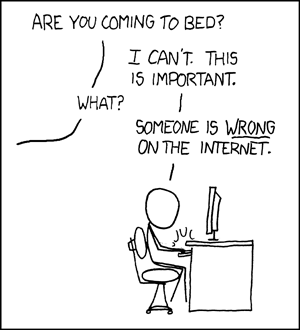
\includegraphics{images/duty_calls}
\caption{Why we need this book?\\ \ccbync~\href{http://xkcd.com/386/}{XKCD}}
\label{xkcd-duty}
}
\end{figure}

\section{Who is this book for?}
You are a Java developer who has written a number of complex programs already, you know how to set up your development environment whether it is an \ac{IDE} or a command line and text editor. You are happy using Maven to manage your code (or at least willing to learn) and you have a interest in geographic problems (or your boss has). However, you are smart and you don't want to have to write a whole geographic library for yourself from scratch. You have no time or energy to look up the Shapefile white paper \citep{ESRI1997} to see how to read your data in, or work out the projection needed to make the map equal area. 

So to make your life easier you've picked an existing library but now you have to learn how that works. This book will help you solve common problems using the \GeoTools library.

The joy of Java programming is that it doesn't matter if you use a Linux machine, a windows box or even a Mac. But beware many parts of the \GeoTools library depend on the AWT and the Java Service Provider mechanism neither of which work on Android devices at the time of writing, so if you want to write Android applications you will need to find another library. That's not to say you can't take some of the code and techniques shown here on Android just that there is a fairly good chance that it will not work as is.
 
\section{A brief history of \GeoTools}
Once upon a time, when I was a newish (and keen) post--doctoral researcher in the \ac{CCG} at the University of Leeds there was a younger (and keener) Master's student call James Macgill who wanted to investigate swarms of agents moving around a map. The current state of the art \ac{GIS} system was unable to do more than draw a simple map. The ``obvious'' solution was to write our own \ac{GIS} system and so \GeoTools was born. Version 1 of the library was really intended for internal use only but news of leaked out and people (like \ac{TOPP} started to use it). Overtime a user community developed, and then they started wanting bug fixes and new features! It was terrible, as by now both of us had other jobs to do and very little spare time for \GeoTools. At the same time it was becoming apparent that there were some design choices that would make extending the library any further difficult, so we took the only sensible course of action and abandoned the project. We then replaced \GeoTools--1 with \GeoTools--2, which was redesigned to incorporate all (or at least some of) the lessons we had learned in \GeoTools--1. 

\GeoTools--2 was built on a generic feature definition, to start with it only supported \ac{OGC} Simple Features, but later when users needed complex features it was (relatively) easy to add support for them. We also switched from using Ant to Maven to manage the build and started to produce modular jar files to allow users to pick and choose the parts they wanted to use. We also recruited a bunch of new developers from \ac{TOPP} and Refractions Research who were building the GeoServer WMS Server and the UDig editor respectively. 

After a while it became clear that \GeoTools--3 was never going to arrive (or it is a long way in the future) so the version of the \GeoTools library moved from 2.7.x to 8.0. This book has been developed against version ${geotools.version} of the library.

\chapter{Introduction}\label{introduction}

\section{Getting Started}
I'm going to make the assumption that as a Java developer who already have a favourite set of development tools and are fairly happy in how to use them. To get anywhere with \GeoTools you will need to have Apache Maven installed on your machine. 

In this chapter we will draw a map. The code you will need is shown in \cref{HelloWorld}.
\lstinputlisting[caption={Hello World GIS style},label=HelloWorld]{quickstart/src/main/java/org/geotools/tutorial/quickstart/Quickstart.java}



\chapter{Input, getting the data in to GeoTools}\label{input}
\section{Vector Datasets}\label{vector}
\section{Raster Datasets}\label{raster}
\chapter{Output}
\todo{think of a better title}

\section{Introduction}
Once you have your data set up the way you would like you will want 
to export it in some sort of form that allows you to use it.

\section{Working with Geometries}\label{geoms}
\todo{decide where this should go}
Within \GeoTools geometries are represented by \ac{JTS} Geometries that contain the actual positions as Coordinates.
Sometimes when exporting geometries you would like to produce a plain text string that represents the geometry, if for no other reason than it's easier to see what is happening than starting up a debugger. 
This sort of interoperability issue comes up often enough that there is a standard way of doing it (well two in fact). The most common format is \ac{WKT}.

\lstinputlisting[firstline=38,firstnumber=38,lastline=40,label=wkt,caption={Exporting WKT from a geometry}]{../modules/output/src/main/java/org/ianturton/cookbook/output/ExportGeometries.java}

\Cref{wkt} shows just how simple this process is. This will produce output like \cref{wktoutput}. WKT is kept deliberately simple so that writing a program that can read it in or write it out is easy. The standard was originally written by the \ac{OGC} as part of Simple Feature specification, it is now defined in the ISO 13249 ``Information technology -- Database languages -- SQL multimedia and application packages -- Part 3: Spatial'' standard.

\begin{figure}[h]
\begin{spverbatim}
POINT (10.1 22.2) 
LINESTRING (1 1, 2 3, 4.4 5.2)
POLYGON ((1 1, 2 3, 4.4 5.2, 1 1))
MULTIPOLYGON (((1 1, 2 3, 4.4 5.2, 1 1)), 
    ((10 10, 20 30, 40.4 50.2, 10 10)))
\end{spverbatim}
\caption{Some examples of WKT}\label{wktoutput}
\end{figure}

One important point to notice is that \spverb!POLYGON! has two parenthesis at the start and end, this allows you to specify holes in your polygon (think islands in a lake) which are represented like \spverb!POLYGON ((35 10, 45 45, 15 40, 10 20, 35 10),(20 30, 35 35, 30 20, 20 30))!. 

\section{Creating an Image of the Map}
Assuming that you have created a map that you like with the correct styling and area of interest 
set then you might want to produce a picture of it. \Cref{save} shows how to do this.

\lstinputlisting[firstline=27,firstnumber=27,label=save,caption=Save a picture of the map.]{../modules/output/src/main/java/org/ianturton/cookbook/output/SaveMapAsImage.java}

\section{Create a New Shapefile}

\lstinputlisting[firstline=40,firstnumber=40,label=shapefile,caption=Save a shapefile.]{../modules/output/src/main/java/org/ianturton/cookbook/output/WriteShapefile.java}


\chapter{Querying, Filtering and Sorting: finding what you need}\label{filters}
\section{Creating and running a query}
\section{Filters}
\subsection{OGC Filters}
\subsection{CQL Filters}
\section{Sorting your results}
\chapter{Styling: How to make a pretty map.}\label{styling}
\section{Introduction}
Try to read \cite{Peterson2012} to see how cartography is really done.
\section{Colouring Features}
\section{Line Styles}
\section{Fonts}
\chapter{Projections}
\section{Introduction}
Why we need to worry about projections? I'm going to let you in on a geographic secret ``the world is round'' -- sadly most of the maps we draw are \textbf{flat}. This leaves us with a problem, as anyone who has ever tried to gift wrap a globe knows, it's hard to make a curved surface and a flat sheet match up. 

As the ever helpful XKCD points out in \cref{xkcd-projections} there are a lot of projections.

\todo{make this image narrower}
\begin{figure}[htbp]
{%
\setlength{\fboxsep}{0pt}%
\setlength{\fboxrule}{1pt}%
\fbox{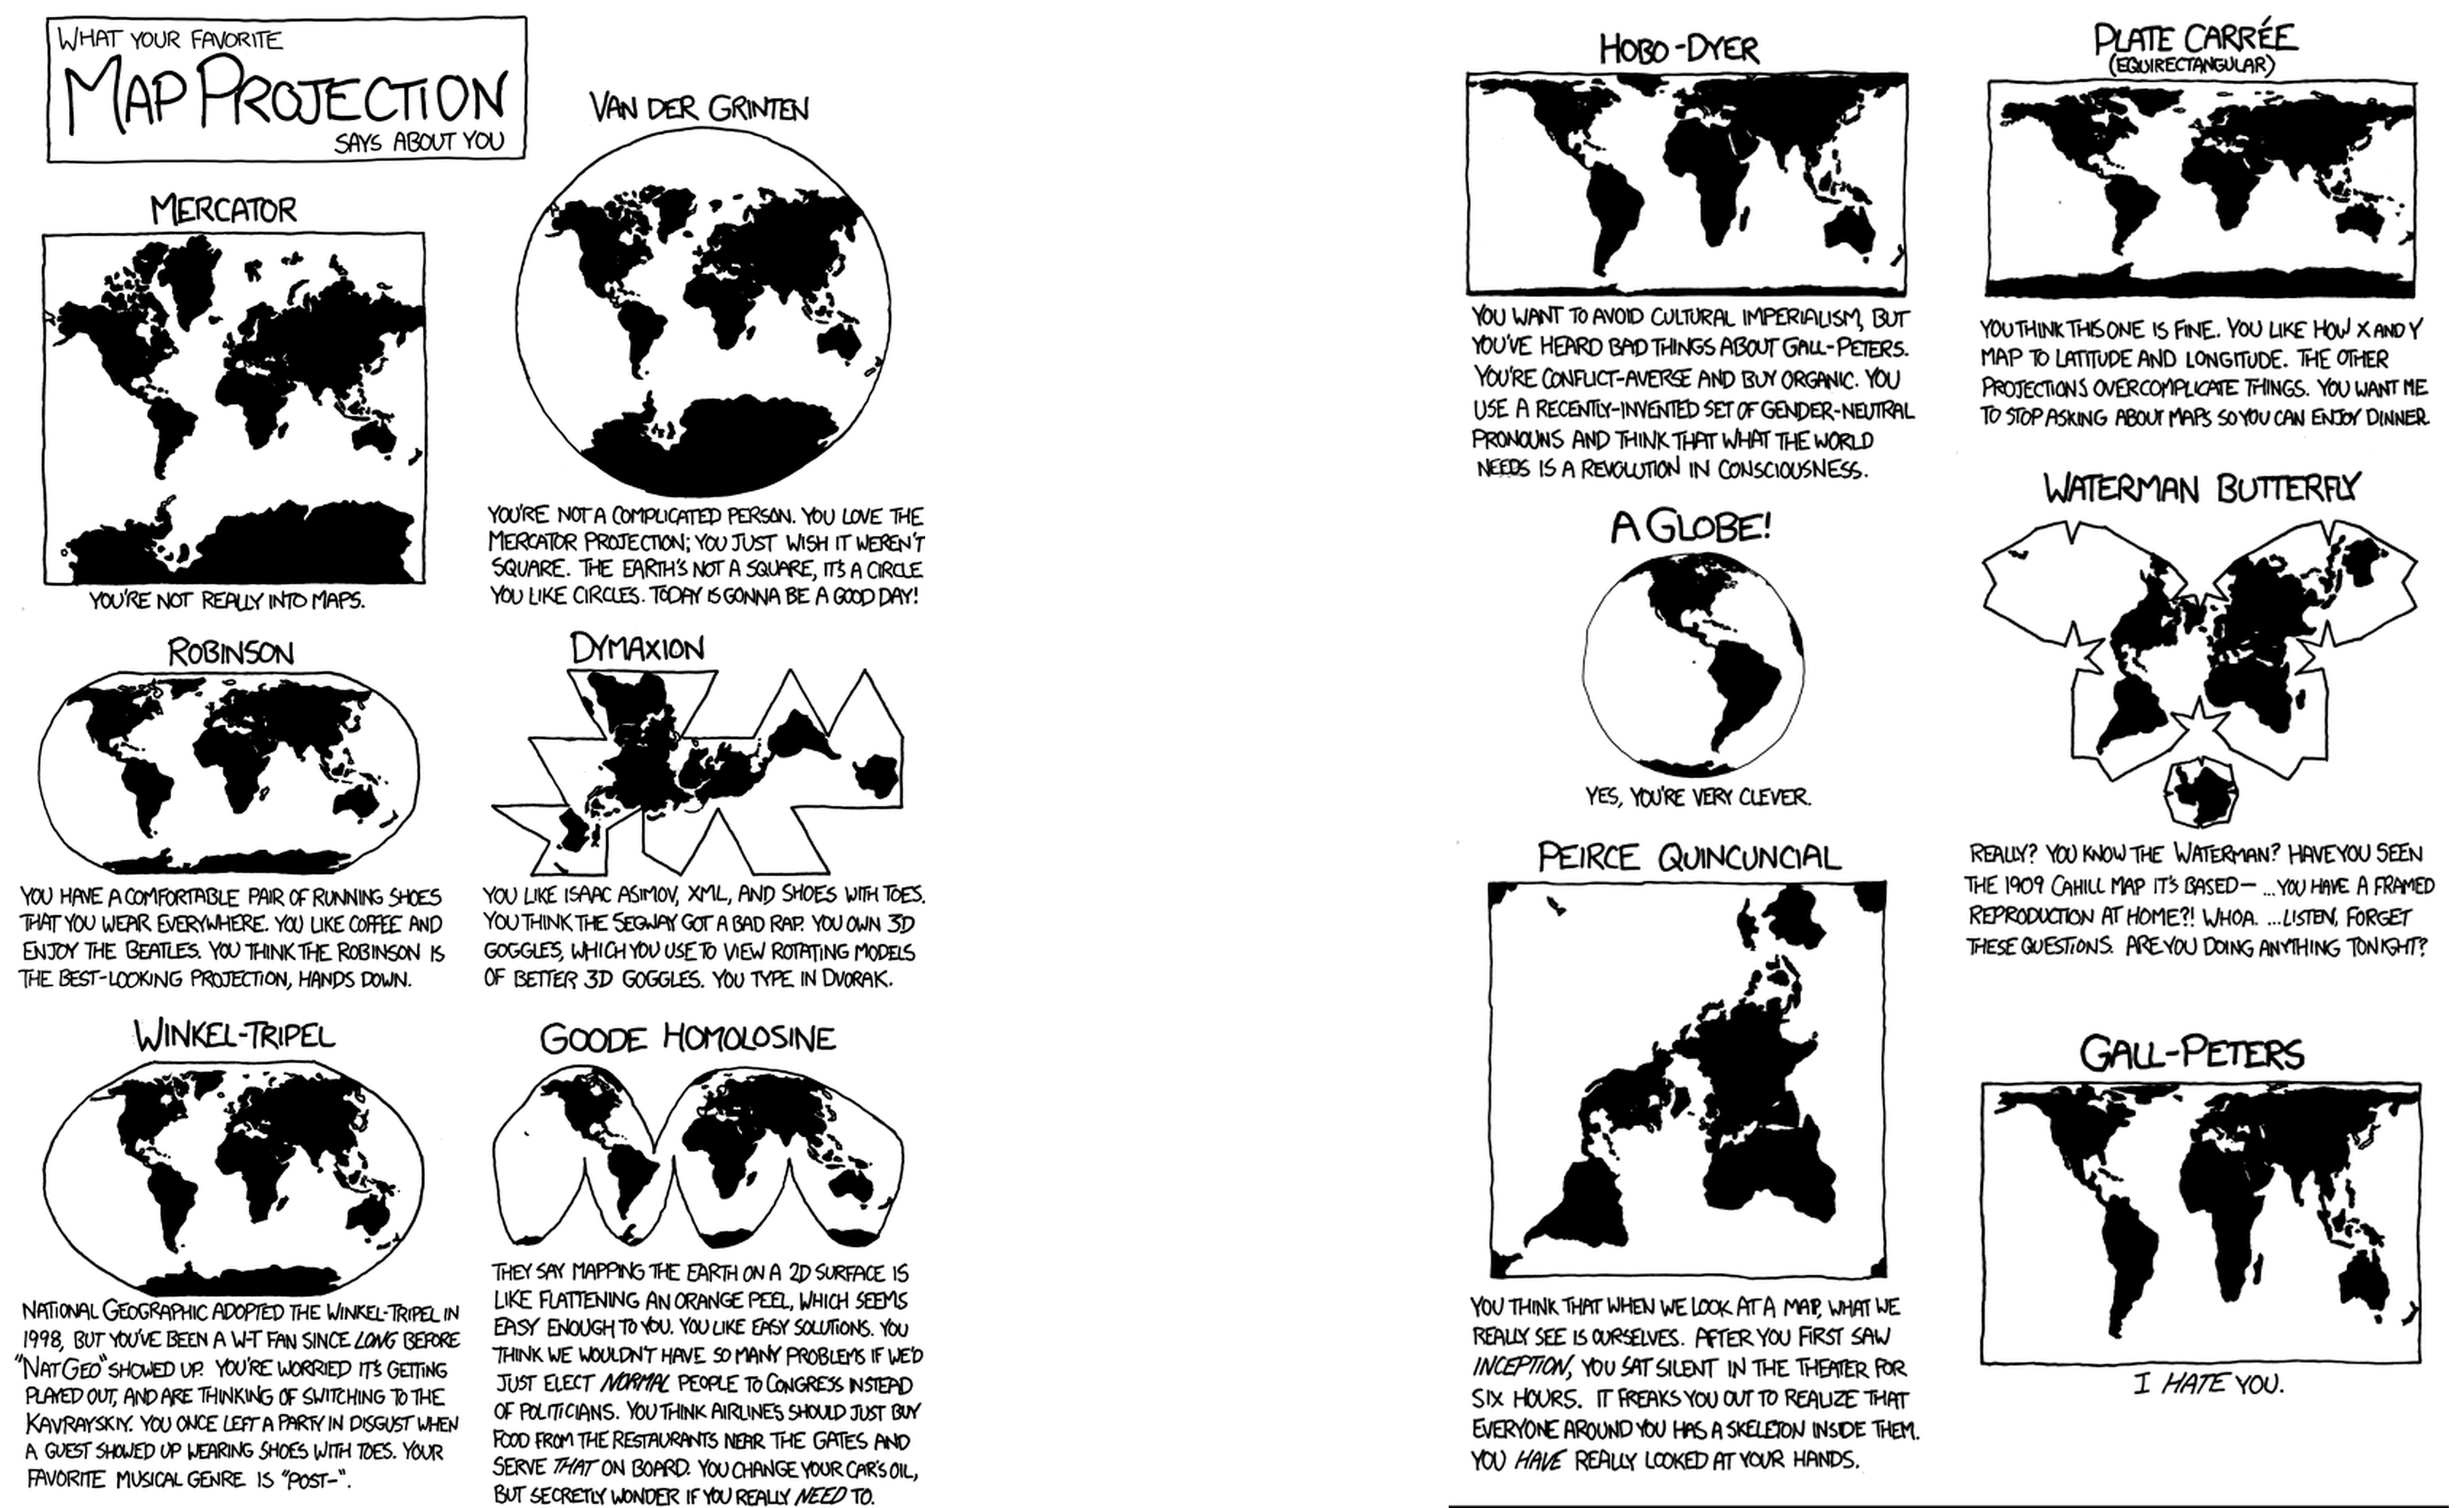
\includegraphics[width=\textwidth]{images/projections2}}%
}%

\caption{A quick introduction to projections\\ \ccbync~\href{http://xkcd.com/977/}{XKCD}}
\label{xkcd-projections}
\end{figure}

Before you go too deep into the world of projections you should download and (at least) skim \cite{snyder}. This will give you access to all the helpful maths that \GeoTools encodes for you (or if you are unlucky that you will need to add a new projection to the library).

\section{How to reproject features in \GeoTools}
\section{How to choose a ``good'' projection}
\chapter{Distances  and GeoFencing}



\lstinputlisting[firstline=21,firstnumber=21,caption=How to calculate the distance between two points.]
{distances/src/main/java/org/ianturton/cookbook/distances/OrthodromicDistance.java}
\label{distance1}

\todo{add the rest of the chapters as includes}
\chapter{Going Further}
\bibliographystyle{plainnat}
\bibliography{refs}
% this contains the acronyms - which for some reason doesn't work at the front.
\cleardoublepage
\chapter*{Acronyms}
\begin{acronym}[XXXXX]
\acro{OGC}{Open Geospatial Consortium}
\acro{JTS}{Java Topology Suite}
\acro{WKT}{Well Known Text}
\acro{WKB}{Well Known Binary}
\acro{ISO}{International Standards Organization}
\acro{CCG}{Centre for Computational Geography}
\acro{GIS}{Geographic Information System}
\acro{TOPP}{The Open Planning Project}
\end{acronym}
\todo{remove this list when finished}
\listoftodos 
\end{document}
